oauthとoauth2は現在比較的流行している二種類の認証方式です。サードパーティでちょうどこの認証を実装しているライブラリがあるのですが、国外で実装されたもので、QQ、weiboといった中国国内のアプリケーション認証はありません。

\begin{lstlisting}[numbers=none]
github.com/bradrydzewski/go.auth
\end{lstlisting}

下のコードはどのようにしてこのライブラリをbeegoの中に導入しoauth認証を実装するか示しています。ここではgithubを例にしています:


\begin{enumerate}
  \item ルーティングを2本追加
\begin{lstlisting}[numbers=none]
beego.RegisterController("/auth/login", &controllers.GithubController{})
beego.RegisterController("/mainpage", &controllers.PageController{})
\end{lstlisting}
  \item 次にGithubControllerログインの画面を処理:
\begin{lstlisting}[numbers=none]
package controllers

import (
    "github.com/astaxie/beego"
    "github.com/bradrydzewski/go.auth"
)

const (
    githubClientKey = "a0864ea791ce7e7bd0df"
    githubSecretKey = "a0ec09a647a688a64a28f6190b5a0d2705df56ca"
)

type GithubController struct {
    beego.Controller
}

func (this *GithubController) Get() {
    // set the auth parameters
    auth.Config.CookieSecret = []byte("7H9xiimk2QdTdYI7rDddfJeV")
    auth.Config.LoginSuccessRedirect = "/mainpage"
    auth.Config.CookieSecure = false

    githubHandler := auth.Github(githubClientKey, githubSecretKey)

    githubHandler.ServeHTTP(this.Ctx.ResponseWriter, this.Ctx.Request)
}
\end{lstlisting}
  \item ログインに成功した後のページ画面を処理
\begin{lstlisting}[numbers=none]
package controllers

import (
    "github.com/astaxie/beego"
    "github.com/bradrydzewski/go.auth"
    "net/http"
    "net/url"
)

type PageController struct {
    beego.Controller
}

func (this *PageController) Get() {
    // set the auth parameters
    auth.Config.CookieSecret = []byte("7H9xiimk2QdTdYI7rDddfJeV")
    auth.Config.LoginSuccessRedirect = "/mainpage"
    auth.Config.CookieSecure = false

    user, err := auth.GetUserCookie(this.Ctx.Request)

    //if no active user session then authorize user
    if err != nil || user.Id() == "" {
        http.Redirect(this.Ctx.ResponseWriter,
                      this.Ctx.Request,
                      auth.Config.LoginRedirect,
                      http.StatusSeeOther)
        return
    }

    //else, add the user to the URL and continue
    this.Ctx.Request.URL.User = url.User(user.Id())
    this.Data["pic"] = user.Picture()
    this.Data["id"] = user.Id()
    this.Data["name"] = user.Name()
    this.TplNames = "home.tpl"
}
\end{lstlisting}
\end{enumerate}

全体の流れは以下のようになります。まずブラウザを開いてアドレスを入力します:

\begin{figure}[H]
   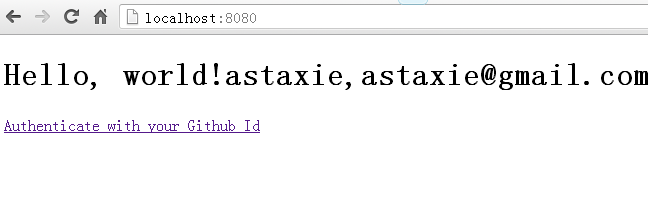
\includegraphics[width=14cm]{14.4.github.png}
   \label{図14.4}
   \caption{ログインボタンを持つトップページの表示}
\end{figure}

次にリンクをクリックすると以下のようなインターフェースが現れます:

\begin{figure}[H]
   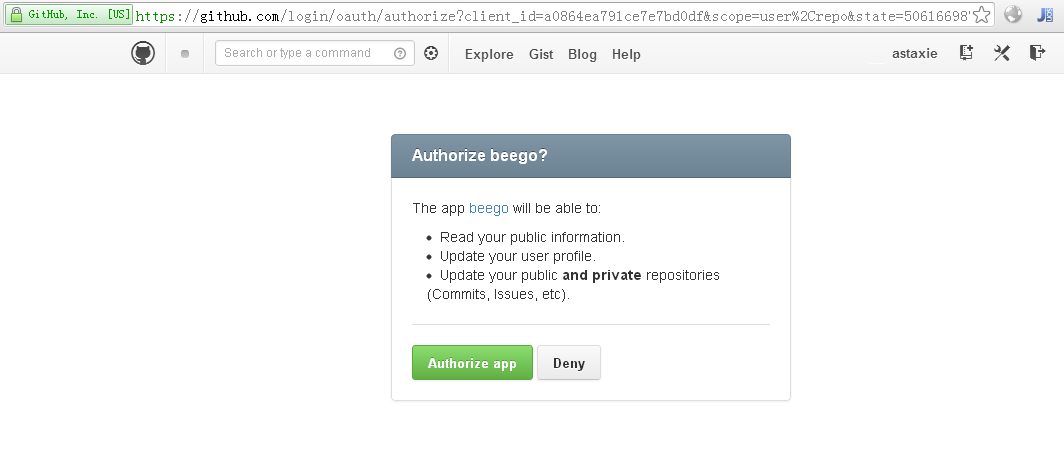
\includegraphics[width=14cm]{14.4.github2.png}
   \label{図14.5}
   \caption{ログインボタンをクリックしてgithubの権限取得ページを表示}
\end{figure}

Authorize appをクリックすると以下のようなインターフェースが現れます:

\begin{figure}[H]
   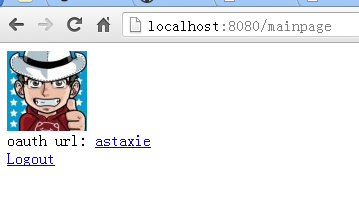
\includegraphics[width=7cm]{14.4.github3.png}
   \label{図14.6}
   \caption{権限取得にログインした後表示される取得済みのgithub情報のページ}
\end{figure}


